\chapter{Configuração do CLP - TB131}
\label{chap:configuracao-clp}


Esta etapa consiste em configurar o CLP, 
de modo a disponibilizar via comunicação serial, acesso aos registradores das entradas e saídas digitais e das entradas e saídas analógicas, por meio de funções do protocolo Modbus RTU. 
No caso deste CLP, 
basta apenas habilitar a porta de comunicação no modo correspondente ao Modbus Servidor RTU (Modbus Slave RTU), que as variáveis digitais já estão disponíveis, enquanto que as analógicas é necessário fazer movimentações de valores entre registradores.


\section{Configuração de comunicação Modbus}

O primeiro passo, caso não haja um projeto criado e aberto, é criar um projeto, a partir do modelo, conforme indicações da Figura \ref{fig:new_project}.

Clique em \textbf{Arquivo} >> \textbf{Novo a partir do modelo...}.

Selecione \textbf{Modelo\_DU350\_DU351\_v110} >> \textbf{Abrir}.

\begin{figure}[ht!]
	\centering
	\Caption{\label{fig:new_project}Criando um novo projeto}
	\UECEfig{}{
		\fbox{\includegraphics[width=15.6cm]{figuras/tb131-new_project }}
	}{
		\Fonte{Elaborado pelo autor}
	}
\end{figure}

Em seguida, clique com o \textbf{botão direito do mouse} em \textbf{POUs}.

Selecione \textbf{Acrescentar objeto...}. 

Selecione \textbf{Programa}, a linguagem Ladder \textbf{LD} e \textbf{OK}, 
conforme indicações da Figura \ref{fig:new_prg}.



\begin{figure}[ht!]
	\centering
	\Caption{\label{fig:new_prg}Acrescentando objeto - Programa em Ladder}
	\UECEfig{}{
		\fbox{\includegraphics[width=15cm]{figuras/tb131-new_prg}}
	}{
		\Fonte{Elaborado pelo autor}
	}
\end{figure}




Após a criação do projeto, a Figura \ref{fig:configAnalog} ilustra os passos para a configuração da comunicação com o protocolo Modbus. 


Acesse a aba \textbf{Recursos} conforme \textbf{indicador 1}.

Clique em \textbf{Configurações do CP} conforme \textbf{indicador 2}.

Na janela central aparecem opções na expansão da \textbf{Configuração do CP}: 

\textbf{Comunicação}, 
\textbf{Barramentos} e 
\textbf{Eventos externos}.

\begin{figure}[ht!]
	\centering
	\Caption{\label{fig:configAnalog}Configuração de parâmetros analógicos}
	\UECEfig{}{
		\fbox{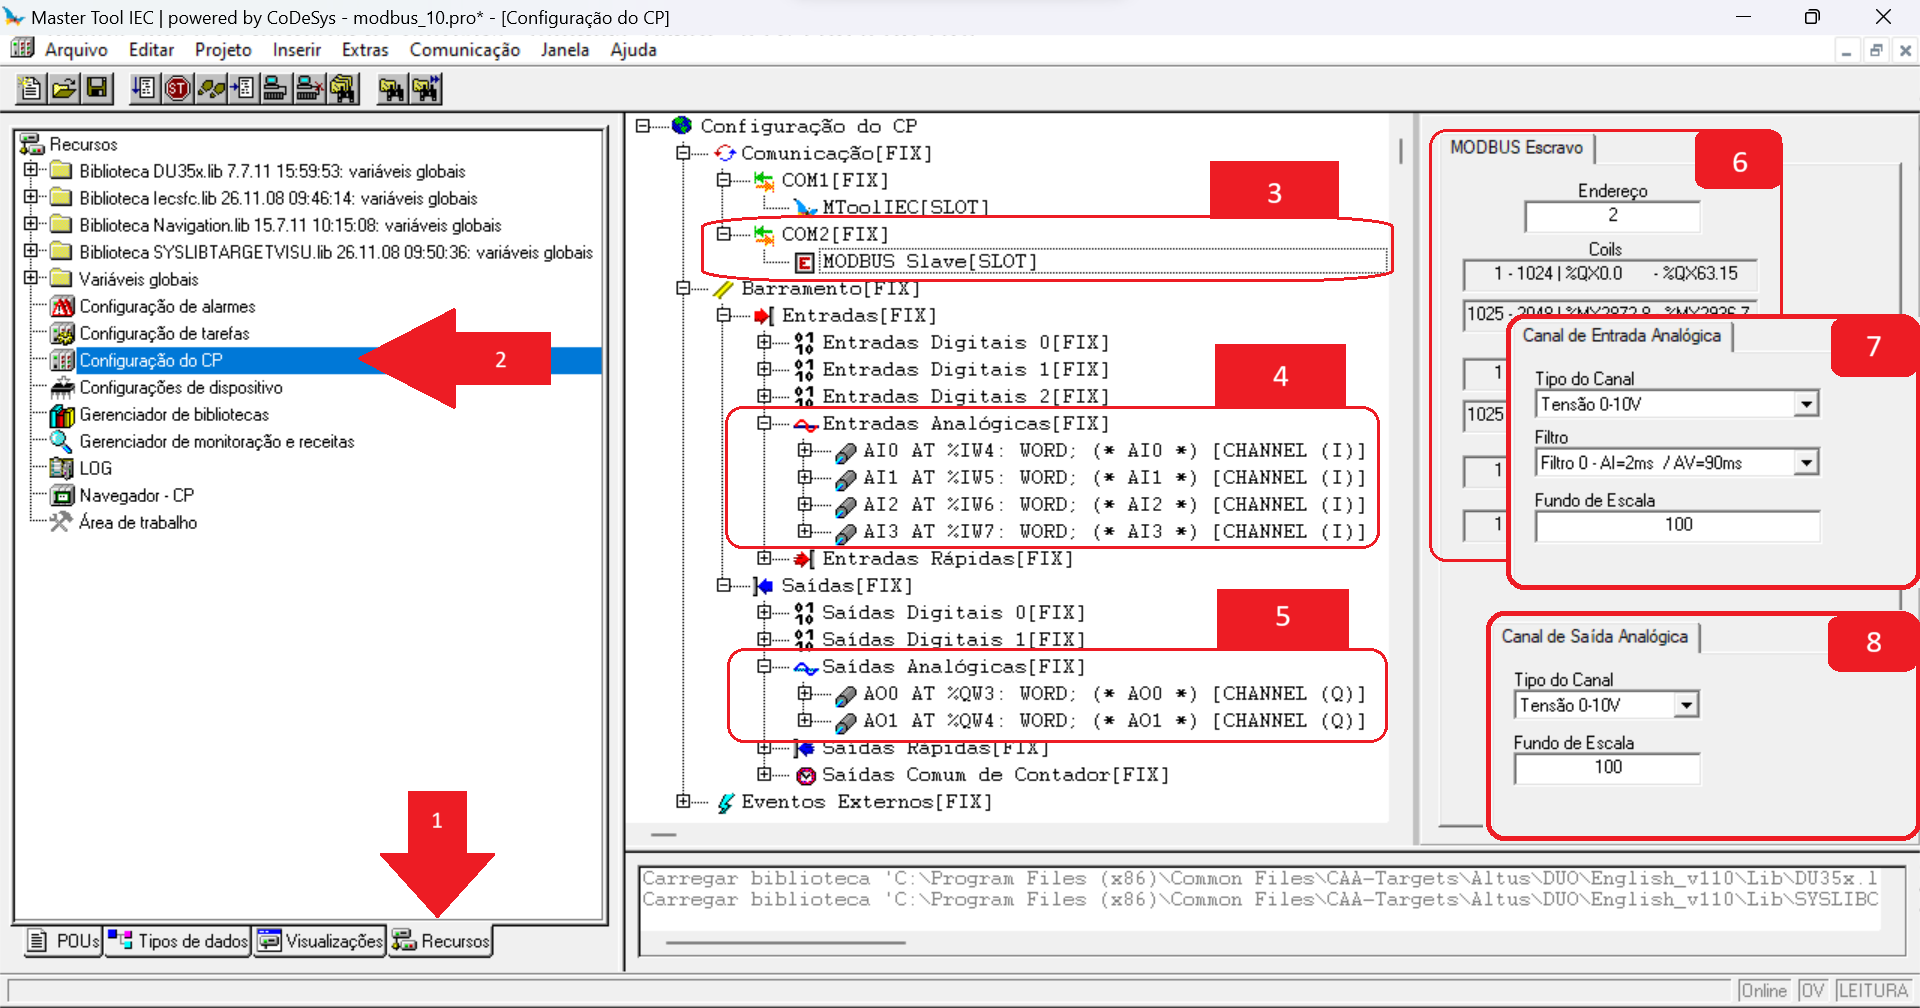
\includegraphics[width=15cm]{figuras/tb131-configAnalogModbus-n}}
	}{
		\Fonte{Elaborado pelo autor}
	}
\end{figure}


Ao expandir a opção \textbf{Comunicação}, abrem-se duas opções: \textbf{COM1} e \textbf{COM2}, sendo esta a ser configurada como \textbf{Modbus Slave}, conforme \textbf{indicador 3}. 
Como parâmetro do servidor modbus (slave), temos apenas que configurar o seu endereço, conforme \textbf{indicador 6}. 
Os demais dados são do mapeamento dos endereços das \textit{IOs} e da memória em relação às funções do protocolo utilizado.

Em \textbf{Barramento} pode-se expandir e acessar 
\textbf{Entradas} e \textbf{Entradas Analógicas}, 
conforme \textbf{indicador 4}. 
São listadas as quatro entradas analógicas (\textbf{AI0, AI1, AI2 e AI3}) e seus respectivos endereços (\textbf{\%IW4, \%IW5, \%IW6 e \%IW7}). 
Ao clicar sobre a linha de qualquer uma das entradas, é possivel configurar o canal, conforme \textbf{indicador 7}, 
para \textbf{Tensão 0-10V}, \textbf{Corrente 0-20mA}, \textbf{Corrente 4-20mA} ou ainda \textbf{Canal Desabilitado}. 
Como queremos utilizar o potenciômetro denominado \textbf{AV0}, 
que está conectado ao canal \textbf{AI0}, 
seleciona-se a opção de \textbf{Tensão 0-10V}. 
A opção de filtro é irrelevante no momento, 
bastando agora setar a opção de \textbf{Fundo de escala} para \textbf{100}. 
Este valor é arbitrário, apenas para fins didáticos, pois seu valor depende da variável do processo que está sendo monitorada.


Em \textbf{Barramento}, pode-se expandir e acessar 
\textbf{Saídas} e \textbf{Saídas Analógicas}, 
conforme \textbf{indicador 5}. 
São listadas 2 saídas analógicas, \textbf{AO0} e \textbf{AO1}, 
alocadas nos endereços \textbf{\%QW3} e \textbf{\%QW4}. 
Da mesma forma que para as entradas, 
ao clicar sobre qualquer linha de uma das saídas, 
é possível configurar o tipo de canal e o fundo de escala, conforme \textbf{indicador 8}. 

Note que todos os canais, analógicos e digitais, são independetes entre si, e possuem seus valores alocados em variáveis do tipo WORD. 





\section{ Declarando variáveis e espelhando variáveis às funções modbus}


\begin{figure}[ht!]
	\centering
	\Caption{\label{fig:insert_function_en}Inserção de funções para manipulação de dados}
	\UECEfig{}{
		\fbox{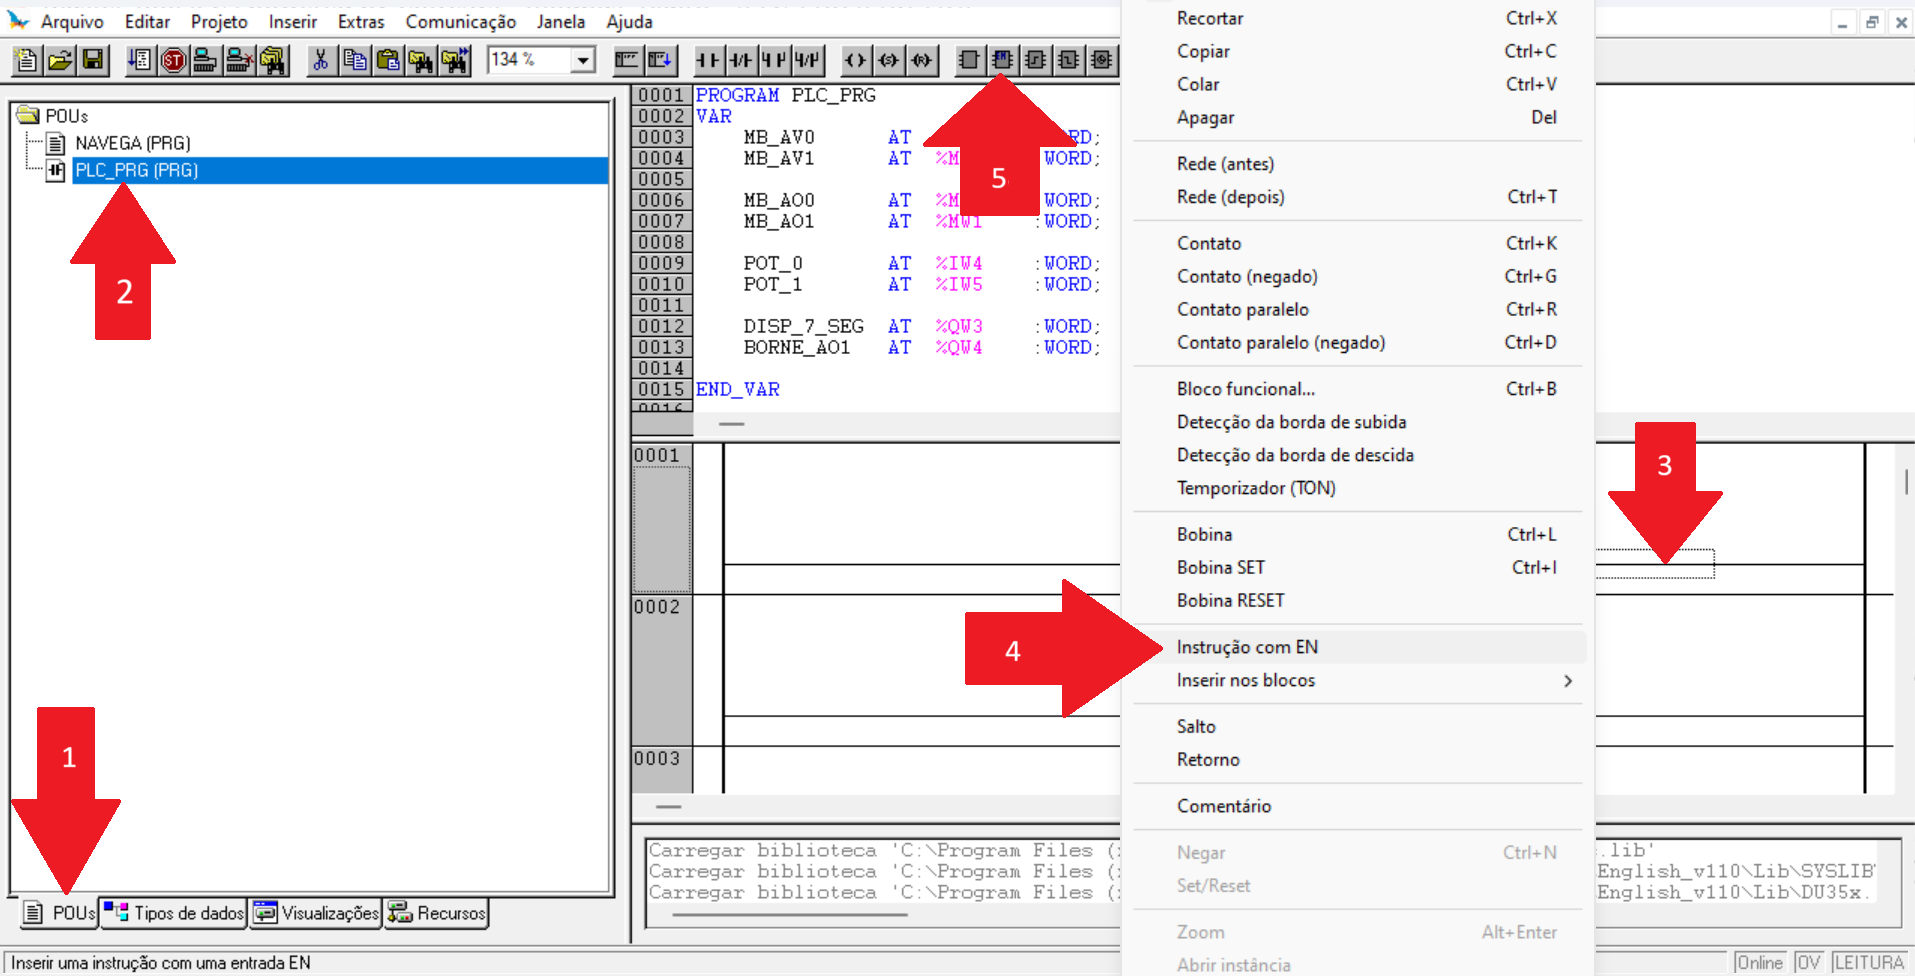
\includegraphics[width=14cm]{figuras/tb131-insert_function_en-n}}
	}{
		\Fonte{Elaborado pelo autor}
	}
\end{figure}


Após a definição da porta e do protocolo de comunicação, 
e da identificação dos canais de entrada e saída analógicos, 
retorna-se à aba do programa, 
conforme \textbf{indicação 1} da Figura \ref{fig:insert_function_en}, 
clicando na \textbf{indicação 2}.


As variáveis utilizadas podem ser definidas conforme forem sendo inseridas e utilizadas no código, ou ainda pode-se declarar todas as variáveis antes de iniciar a inserção dos blocos do programa. 


A Figura \ref{fig:declaracao_vars} ilustra a declaração de variáveis conforme serão utilizadas. 
Note que as variáveis, cujos nomes começam com 'MB\_', 
correspondem ao endereços do protocolo modbus. 
As demais variáves correspondem aos periféricos do TB131, 
POT para os potenciômetros e as saídas com os nomes explícitos: 
DISP\_7SEG e BORNE\_AO1.


\begin{figure}[ht!]
	\centering
	\Caption{\label{fig:declaracao_vars}Declaração de variáveis}
	\UECEfig{}{
		\fbox{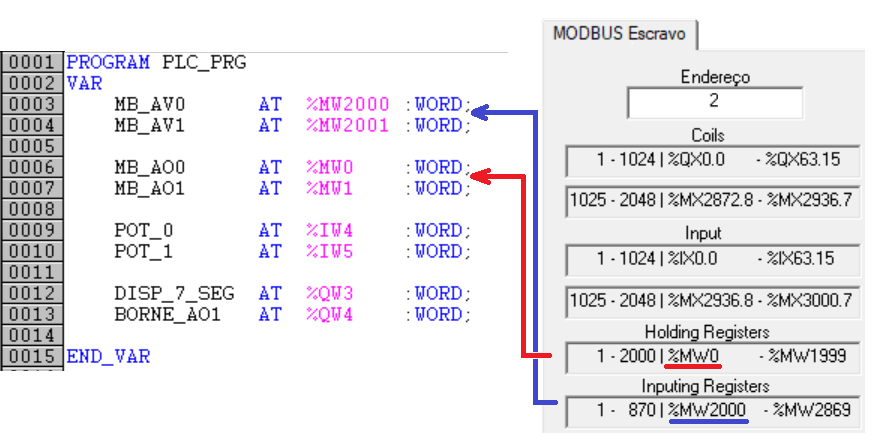
\includegraphics[width=14cm]{figuras/tb131-progCLP_vars-n-m}}
	}{
		\Fonte{Elaborado pelo autor}
	}
\end{figure}


Após a declaração das variáveis, 
é o momento de inserir no programa, 
os elementos que farão a movimentação dos dados 
dos endereços de hardware para 
os endereços das funções da comunicação modbus. 

O \textbf{indicador 3} da Figura \ref{fig:insert_function_en}, 
ilustra o local a ser inserida uma instrução com habilitação, 
ao clicar com o botão direito do mouse, conforme \textbf{indicador 4}. 
Ou ainda, ao clicar no ícone do \textbf{indicador 5}.


A Figura \ref{fig:funcoes_analog} ilustra o uso da função 
\textbf{MOVE} para transferir informação das entradas analógicas 
para os endereços correspondetes às funções de leitura no 
protocolo Modbus, bem como, 
dos endereços de escrita das funções Modbus para as saídas analógicas. 

\begin{figure}[ht!]
	\centering
	\Caption{\label{fig:funcoes_analog}Espelhamento de parâmetros analógicos para comunicação Modbus}
	\UECEfig{}{
		\fbox{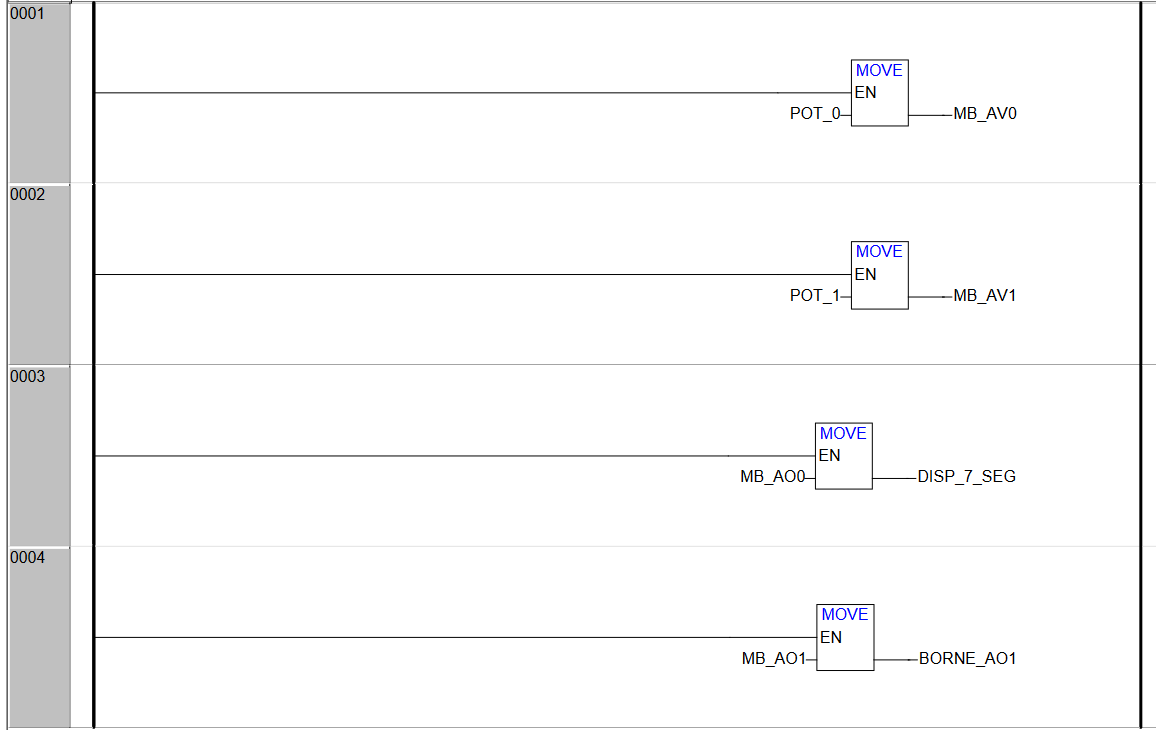
\includegraphics[width=14cm]{figuras/tb131-progCLP_analogReg}}
	}{
		\Fonte{Elaborado pelo autor}
	}
\end{figure}


Note que em todos os casos, 
a entrada \textbf{EN}, habilitação, 
está conectada e ligada direto à fonte de sinal, 
tornando todos os blocos habilitados de forma ininterrupta. 


Na primeira rede do programa, 
acontece a transferência do \textbf{POT\_0}, 
que corresponde ao endereço \textbf{\%IW4}, 
ou seja, a entrada analógica \textbf{AI0} para o \textbf{MB\_AV0},
declarada no endereço \textbf{\%MW2000}, 
que de acordo com a Figura \ref{fig:com_modbus_slave_address}, 
é o primeiro endereço da função \textbf{\textit{Inputing Register}}.

Na segunda rede do programa, 
de forma anaáloga à primeira rede, 
transfere-se o valor da segunda entrada analógica para o endereço correspondente Modbus.

Na terceira rede do programa, 
ocorre a transferência de \textbf{MB\_AO0}, 
que corresponde ao endereço \textbf{\%MW0}, 
primeiro endereço da função Modbus 
\textbf{\textit{Holding Register}}. 
Como recebedor deste valor via comunicação Modbus temos o 
\textbf{DISP\_7\_SEG}, alocado no endereço \textbf{\%QW3}, 
vinculado ao par de displays de sete segmentos no TB131. 

Na quarta rede do programa, 
de forma análoca à terceira rede, 
a trasferência do segundo endereço da função modbus para a segunda saída analógica do CLP, 
conectada no borne \textbf{AO1}, que pode ser verificada com o auxílio da utilização de um votímetro. 




\section{Compilação do programa}

Após todas as variáveis estarem declaradas e devidamente carregadas, 
recomenda-se realizar a compilação do programa. 
A compilação consiste no processamento do que foi realizado até o momento, 
de forma a garantir a consistência da sintaxe do projeto. 

Para realizar a compilação do projeto, 
acesse a aba \textbf{Projeto}, 
conforme \textbf{indicador 1} na Figura \ref{fig:compilacao} 
e clique em \textbf{Compilar tudo}, conforme \textbf{indicador 2}. 
Ao final da compilação, deve aparecer a resposta conforme o \textbf{indicador 3}, apresentando \textbf{0 erro(s) e 0 aviso(s)}. 
Caso algum erro seja exibido, verifique o comentário para ter um indicativo do que não está de acordo. 
Corrija e compile tudo novamente. 


\begin{figure}[ht!]
	\centering
	\Caption{\label{fig:compilacao}Compilação do programa}
	\UECEfig{}{
		\fbox{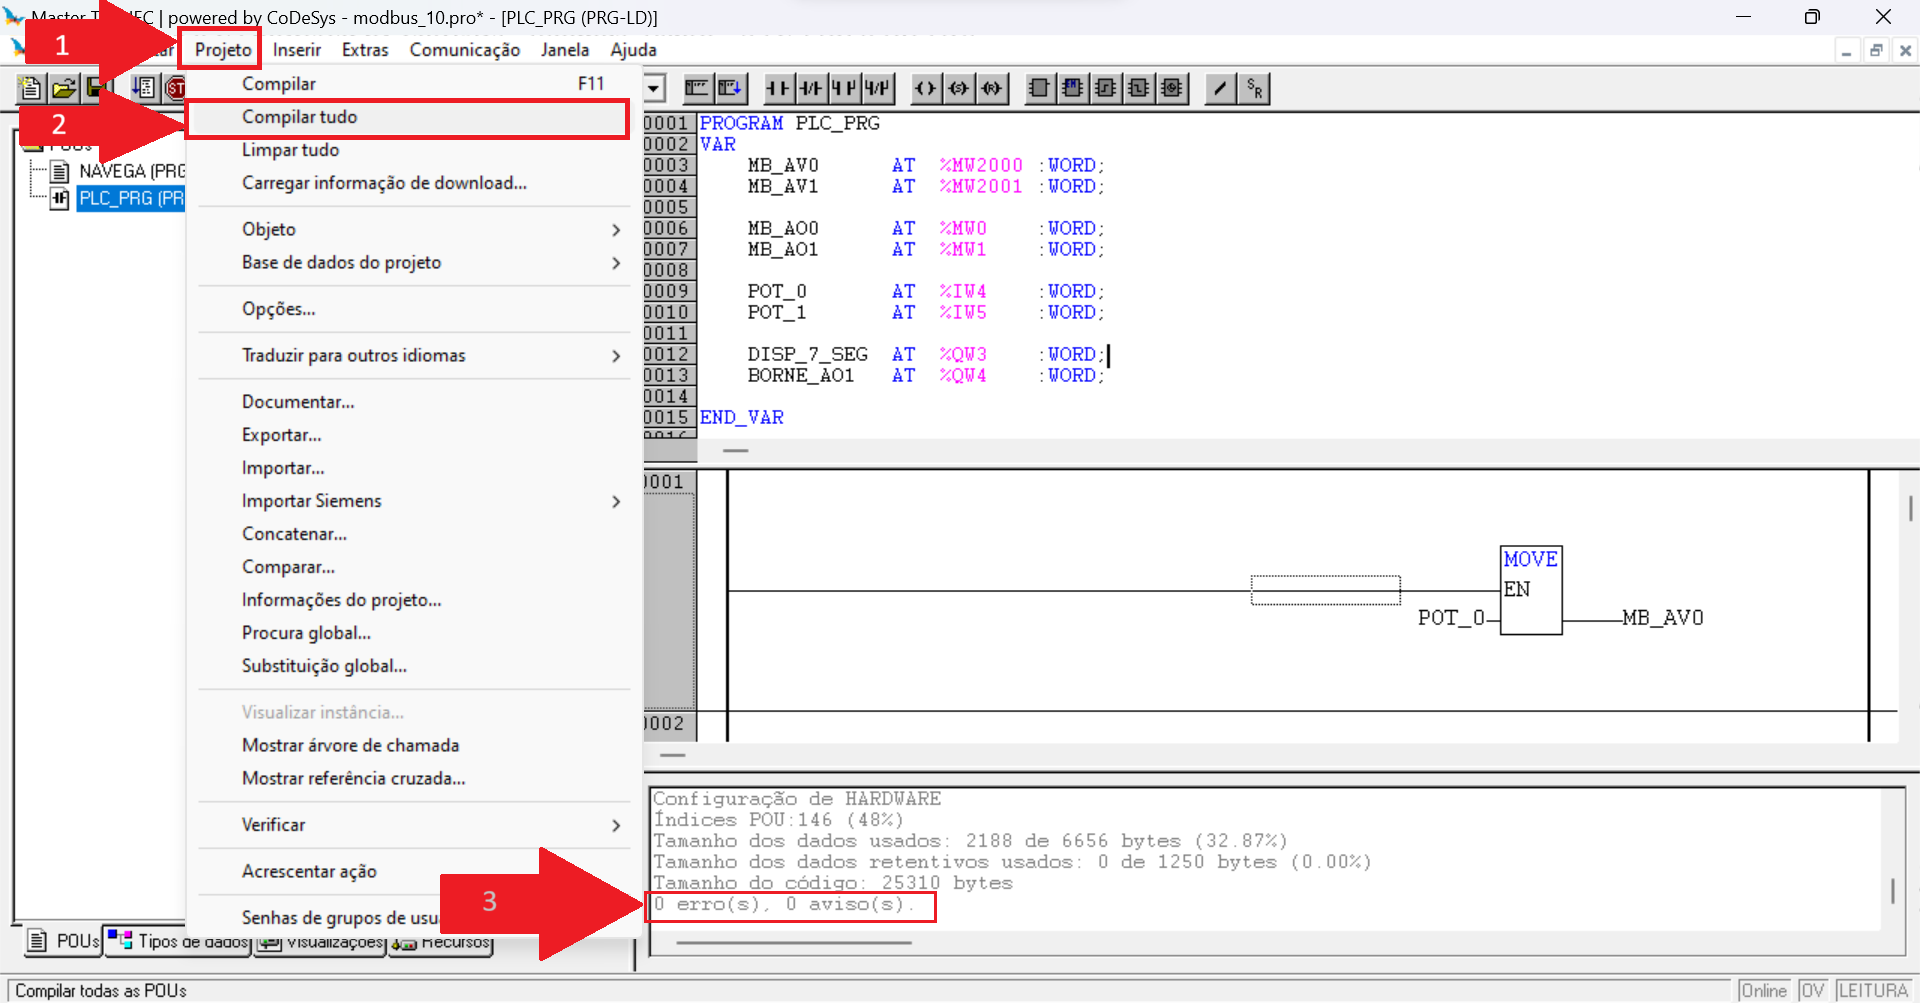
\includegraphics[width=14cm]{figuras/tb131-compile-n}}
	}{
		\Fonte{Elaborado pelo autor}
	}
\end{figure}


Ao clicar na opção \textbf{Compilar}, 
apenas aquilo que foi alterado é compilado, 
o restante do código se mantém. 
Ao clicar em \textbf{Compilar tudo}, 
todos os arquivos auxiliares são reconstruídos, 
e o projeto é processado por inteiro, 
como se não tivesse sido compilado anteriormente. 


\section{Transferência do projeto compilado}

Com o projeto compilado por completo e sem erros, 
é hora de verificar a comunicação entre o computador e o CLP. 

Clique na aba \textbf{Comunicação}, conforme o \textbf{indicador 1} da Figura \ref{fig:parametro_comunicacao}. 

Em seguida verifique se o \textbf{Modo Simulação} está desabilitado, conforme \textbf{indicador 2}. 



\begin{figure}[ht!]
	\centering
	\Caption{\label{fig:parametro_comunicacao}Configuração de parâmetros de comunicação }
	\UECEfig{}{
		\fbox{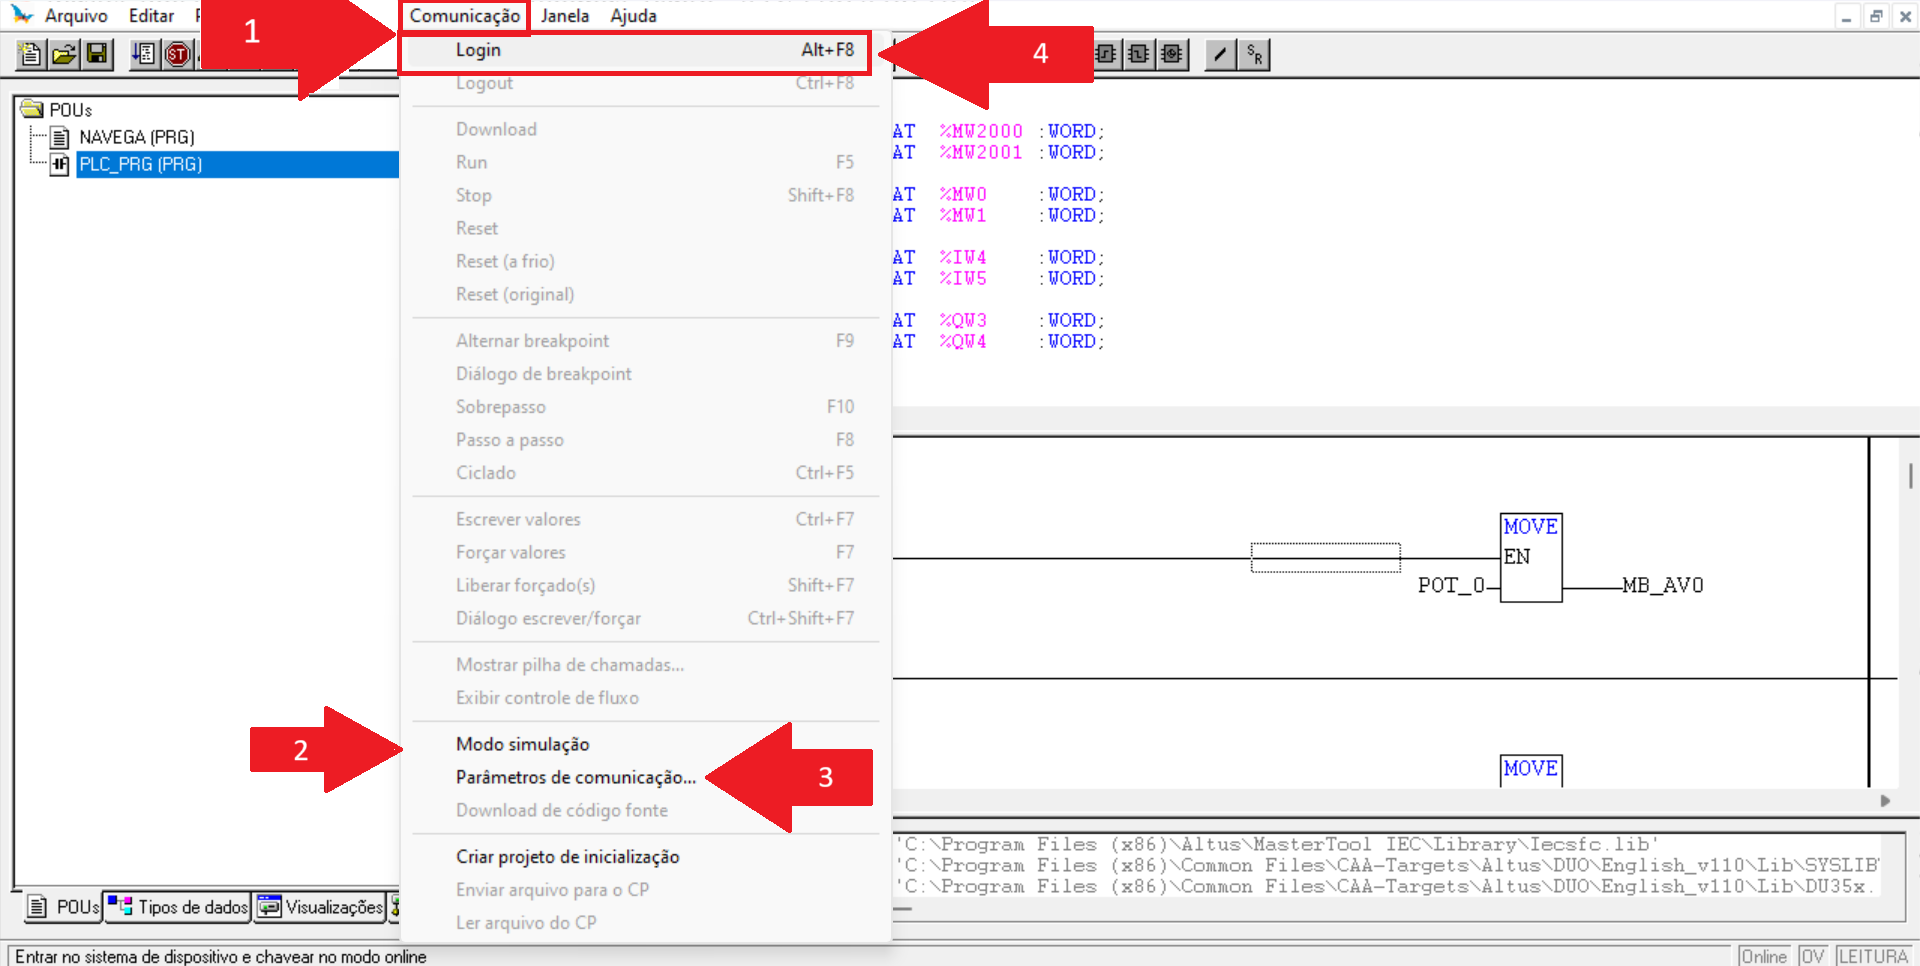
\includegraphics[width=14cm]{figuras/tb131-parametro_comunicacao-n}}
	}{
		\Fonte{Elaborado pelo autor}
	}
\end{figure}


Verifique os parâmetros de comunicação, 
conforme \textbf{indicador 3}.
Estando tudo correto, clique em \textbf{login}, conforme \textbf{indicador 4}. 


\begin{figure}[ht!]
	\centering
	\Caption{\label{fig:param_com_serial}Parâmetros de comunicação da porta Serial}
	\UECEfig{}{
		\fbox{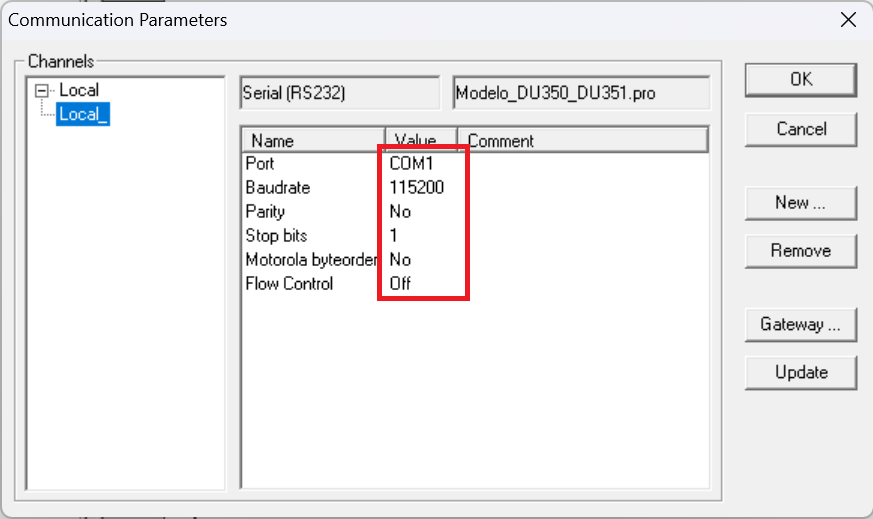
\includegraphics[width=14cm]{figuras/tb131-parametro_comunicacao_set-n}}
	}{
		\Fonte{Elaborado pelo autor}
	}
\end{figure}


Ao realizar o login de um projeto com a compilação diferente do que está gravado no CLP, 
aparece a mensagem para a retransmissão do programa executável, 
de modo a que possa ser realizado o monitoramento em tempo real das variáveis do CLP.


Ao acessar os \textbf{parâmetros de comunicação}, 
deve-se atentar principalmente para a \textbf{porta} e a \textbf{taxa de transmissão (\textit{baud rate})}. 
Para o ajuste desses valores, selecione a variável que se quer alterar com um \textbf{clique duplo} e o ajuste é realizado com as \textbf{setas do teclado}, para cima e para baixo.



\section{Exibir variáveis na IHM integrada - TB131}


Como uma forma redundante, 
as variáveis analógicas são exibidas no display gráfico do CLP. 
A Figura \ref{fig:display_design} ilustra no \textbf{indicador 1} a aba para a composição gráfica da tela. 
O \textbf{indicador 2} aponta para a tela principal, 
que é criada por padrão em todos os projetos. 
Como a exploração deste display está fora do escopo deste trabalho, 
aqui é abordada apenas a inserção de visualização de variáveis. 


\begin{figure}[ht!]
	\centering
	\Caption{\label{fig:display_design}Inserindo tela gráfica no TB131}
	\UECEfig{}{
		\fbox{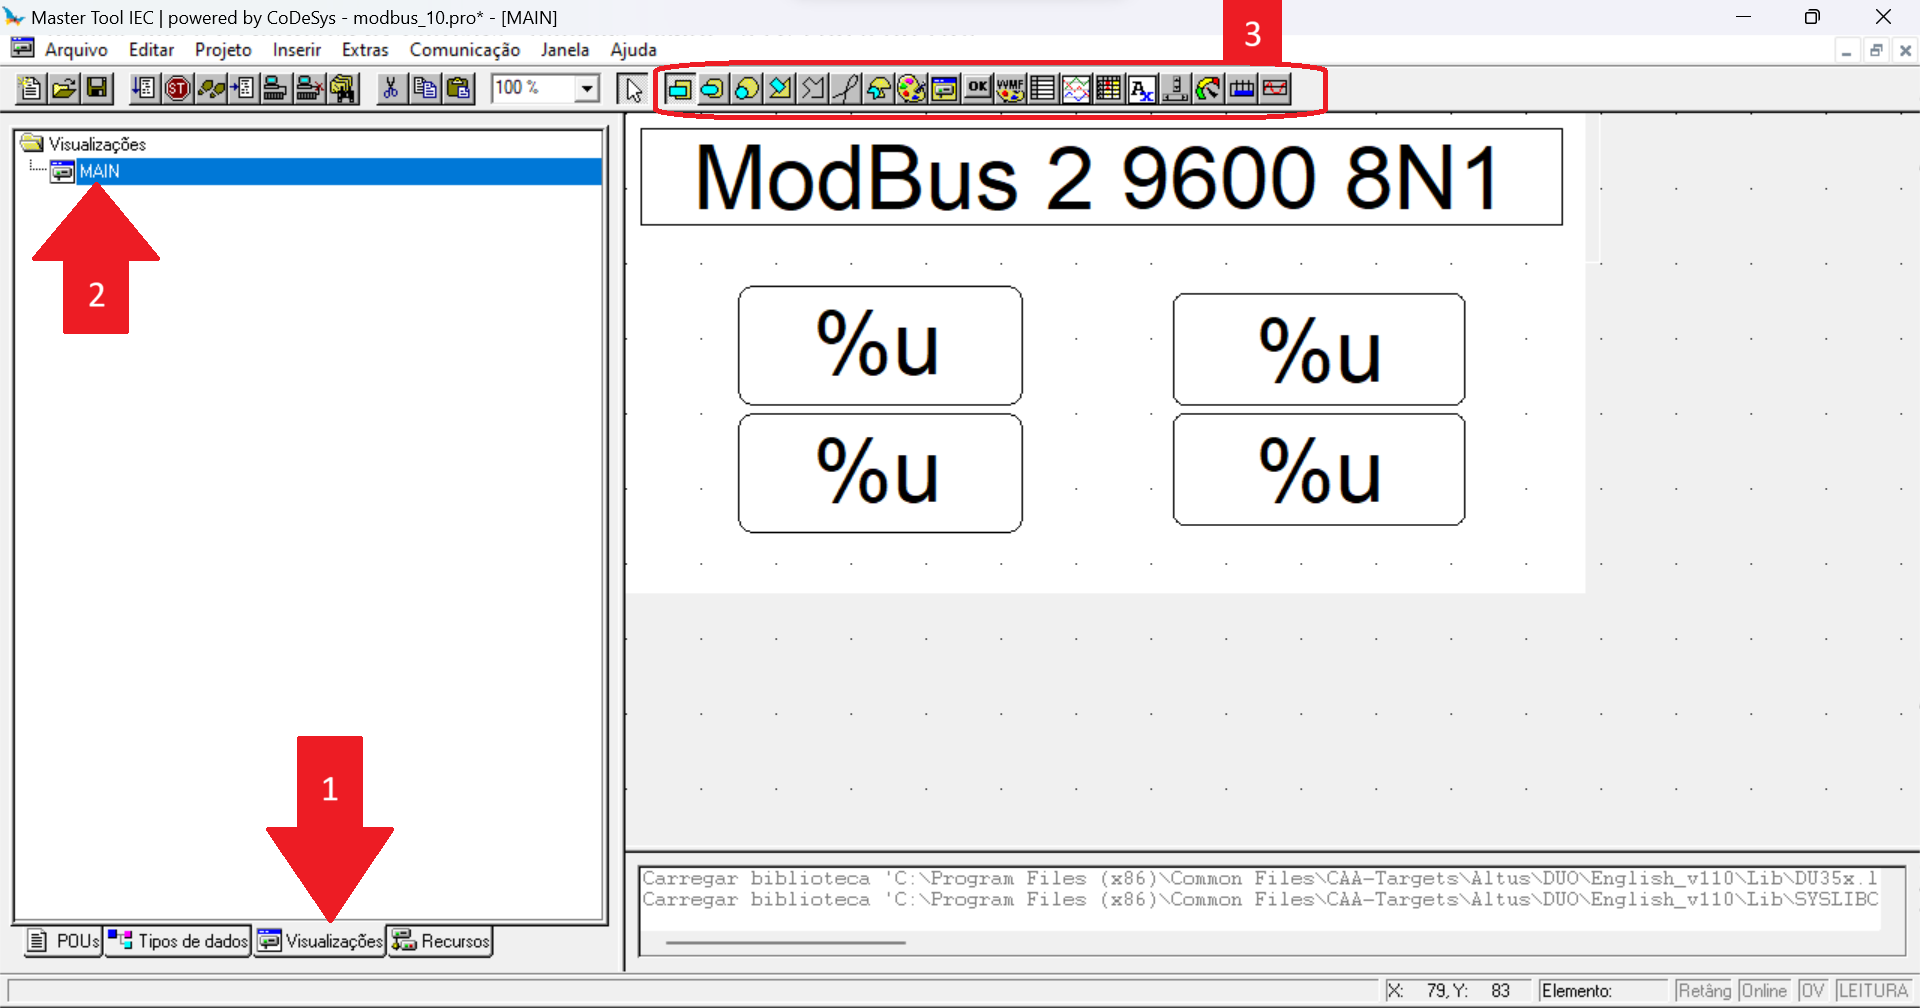
\includegraphics[width=14cm]{figuras/tb131-display_design-n}}
	}{
		\Fonte{Elaborado pelo autor}
	}
\end{figure}


Utilizando basicamente a ferramenta \textbf{Retângulo}, 
que é a primeira ferramenta à esquerda, mostrada pelo \textbf{indicador 3}, são inseridos elementos para o cabeçalho e a exibição das quatro variáveis analógicas utilizadas. 
 
Para o cabeçalho, 
ocorre apenas uma edição com a inserção do texto simples, 
ao clicar sobre o elemento, 
selecionar a opção \textbf{Texto} e na caixa de conteúdo inserir o texto do cabeçalho.
Neste caso foram inseridos os dados básicos da comunicação modbus, 
o número do servidor, \textbf{Slave=2}, 
a taxa de comunicação, \textbf{baud rate = 9600} e o complemento de \textbf{8 bits, sem paridade e um stop bit}, 
representado por \textbf{8N1}.

Para a inserção de variáveis, 
é necessário indicar na caixa de \textbf{Conteúdo} da categoria \textbf{Texto} o formato do dado a ser exibido, 
conforme indicação na Figura \ref{fig:display_var_type}.


\begin{figure}[ht!]
	\centering
	\Caption{\label{fig:display_var_type}Configurando a exibição de um dado numérico}
	\UECEfig{}{
		\fbox{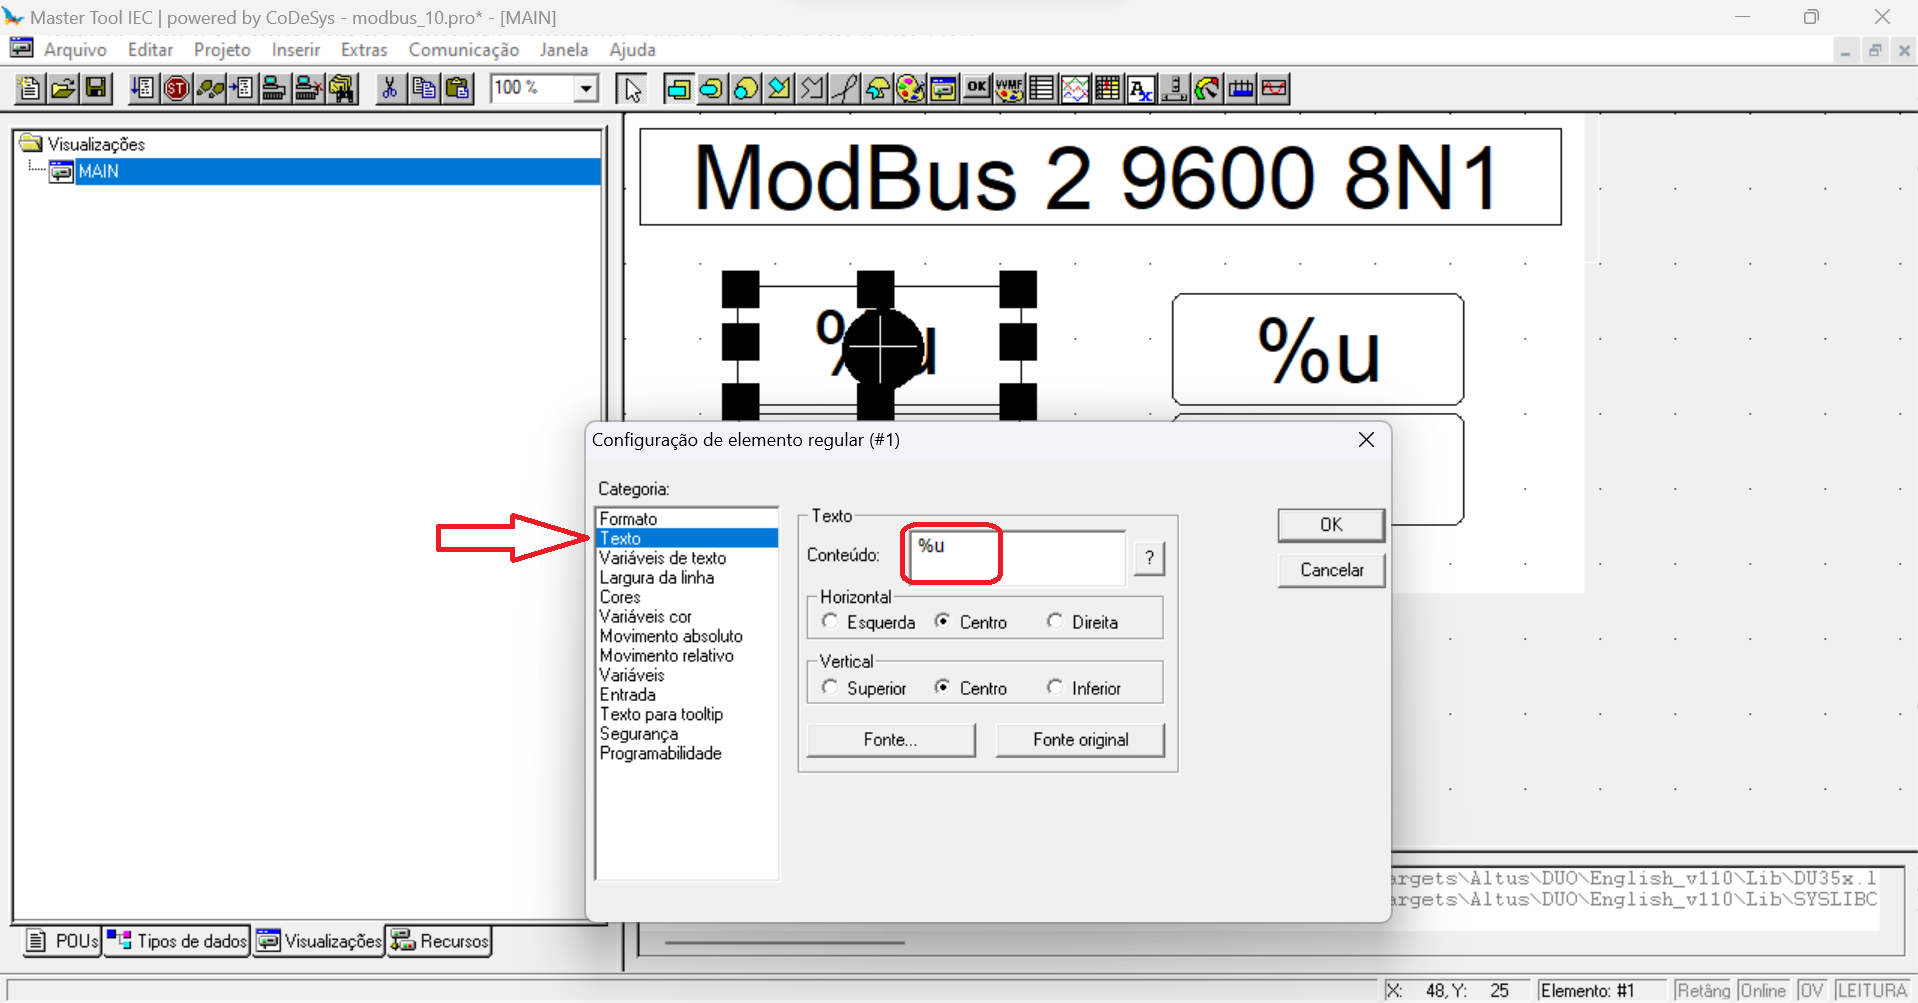
\includegraphics[width=13cm]{figuras/tb131-display_var_type-n}}
	}{
		\Fonte{Elaborado pelo autor}
	}
\end{figure}

Em seguida é necessário indicar a fonte do dado, 
como mostra a Figura \ref{fig:display_var}. 
Em \textbf{Categoria} selecione \textbf{Variáveis} e 
posicione o cursor no campo de edição de \textbf{Texto} 
pressionando em seguida a tecla \textbf{F2}. 
O assistente de entrada é aberto com as \textbf{Expressões de monitoração}. 
Expandindo a opção do programa, como \textbf{indicador 3}, 
são exibidas as variáveis já declaradas no programa, 
conforme destacado pelo \textbf{indicador 4}. 



\begin{figure}[ht!]
	\centering
	\Caption{\label{fig:display_var}Definindo a variável a ser exibida}
	\UECEfig{}{
		\fbox{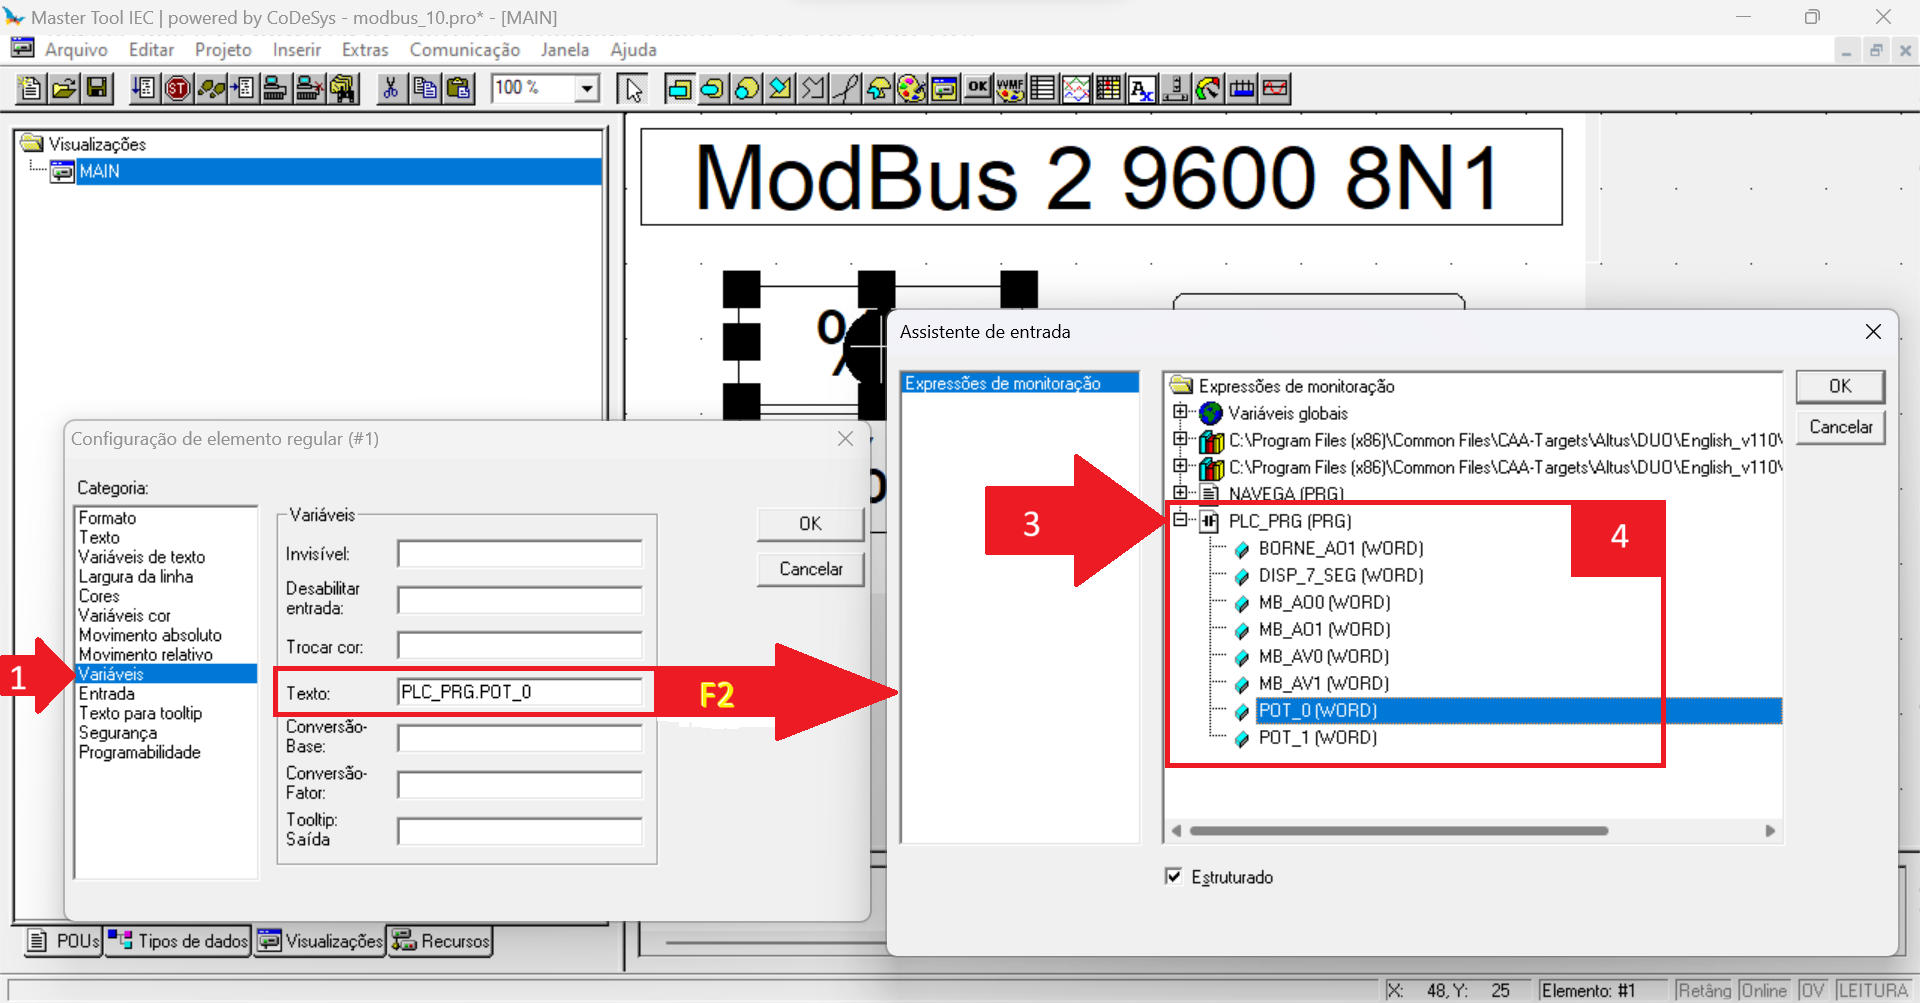
\includegraphics[width=13cm]{figuras/tb131-display_var-n}}
	}{
		\Fonte{Elaborado pelo autor}
	}
\end{figure}

Após variável selecionada é só clicar em 'OK' nas telas em aberto e repita o processo para as demais variáveis que serão exibidas na tela. 
Em seguida, faça a compilação do projeto e o download para carregar o projeto completo no CLP. 


